\documentclass[border=10pt,varwidth=30cm]{standalone}
\usepackage{graphicx,capt-of}
\usepackage{rotating}
\usepackage{multirow}
\usepackage[cm]{sfmath}

\renewcommand{\familydefault}{\sfdefault}

\begin{document}

\begin{figure}
    \centering
    \begin{tabular}{@{}cccc@{}}

        & \multirow{1}{0.15\textwidth}{\centering StarBEAST2}
        & \multirow{1}{0.15\textwidth}{\centering Ecoevolity} \\

        % Row 1
        \multirow{3}{*}[-14em]{\begin{sideways}Estimated\end{sideways}}
        % \multirow{3}{*}[-14em]{\rotatebox{90}{Estimated}}
        & \includegraphics[width=0.15\textwidth]{{../out-sp2-gen4-loc100-len1000/singleton-prob-1.0-starbeast-time}.pdf}
        & \includegraphics[width=0.15\textwidth]{{../out-sp2-gen4-loc100-len1000/singleton-prob-1.0-ecoevolity-time}.pdf}
        % & \begin{sideways}1000 BP\end{sideways} \\
        & \rotatebox{90}{1000 BP} \\
        
        % Row 2
        & \includegraphics[width=0.15\textwidth]{{../out-sp2-gen4-loc200-len500/singleton-prob-1.0-starbeast-time}.pdf}
        & \includegraphics[width=0.15\textwidth]{{../out-sp2-gen4-loc200-len500/singleton-prob-1.0-ecoevolity-time}.pdf}
        & \begin{sideways}500 BP\end{sideways} \\

        % Row 3
        & \includegraphics[width=0.15\textwidth]{{../out-sp2-gen4-loc400-len250/singleton-prob-1.0-starbeast-time}.pdf}
        & \includegraphics[width=0.15\textwidth]{{../out-sp2-gen4-loc400-len250/singleton-prob-1.0-ecoevolity-time}.pdf}
        & \begin{sideways}250 BP\end{sideways} 
        \\

        \multicolumn{4}{c}{\centering True Value} \\
       
    \end{tabular}
\end{figure}

\end{document}